\section{OLED的使用}
\subsection{添加驱动库文件(以SSD1306为例)}
在 PlatformIO 的 Library 中找到驱动库（以 Adafruit 的驱动库为例），点击后添加到自己的工程中。

\begin{figure}[htbp]
    \centering
    \tikzset{
        process/.style={
            rectangle, 
            minimum width=4cm, 
            minimum height=0.8cm, 
            text centered, 
            text width=4.5cm, 
            draw=black, 
            fill=blue!5,
            font=\small
        },
        arrow/.style={thick, ->, >=stealth}
    }

    \begin{tikzpicture}[node distance=1.2cm]
        \node (step1) [process] {1. 进入 PIO Home $\rightarrow$ Libraries};
        \node (step2) [process, below=of step1] {2. 搜索栏输入 ``SSD1306''};
        \node (step3) [process, below=of step2] {3. 选择 Adafruit SSD1306};
        \node (step4) [process, below=of step3] {4. 点击 ``Add to Project''};
        \node (step5) [process, below=of step4] {5. 选择当前工程并点击 Add};

        \draw [arrow] (step1) -- (step2);
        \draw [arrow] (step2) -- (step3);
        \draw [arrow] (step3) -- (step4);
        \draw [arrow] (step4) -- (step5);
    \end{tikzpicture}
    \caption{PlatformIO 添加 SSD1306 驱动库流程}
    \label{fig:pio_lib_add}
\end{figure}

添加完成后，建议检查项目根目录下的 \texttt{platformio.ini} 文件，确认 \texttt{lib\_deps} 选项中已包含 \texttt{adafruit/Adafruit SSD1306}。
\par
接下来，在代码中包含驱动库的头文件，并按照库的使用说明进行初始化和调用相关函数来控制 OLED 显示。
在不知道如何使用的时候，可以参考该库的示例代码，通常在库的安装目录下会有一个 \texttt{examples} 文件夹，里面包含了各种使用示例，可以帮助你快速上手。
亦或者你可以在添加该驱动库的界面查看一下他给的示例代码, 也可以在网上搜索一下相关的使用教程, 以便更好地理解和使用该驱动库。
\par
接下来的代码是初始化OLED显示屏的通用代码,基本不需要做什么修改, 只需要按照你使用的驱动库的要求进行相应的调整即可。
\begin{lstlisting}[language=C]
    #include <Arduino.h>

    #include <SPI.h>
    #include <Wire.h>
    #include <Adafruit_GFX.h>
    #include <Adafruit_SSD1306.h>
    #define SDA_PIN 4
    #define SCL_PIN 5

    Adafruit_SSD1306 oled = Adafruit_SSD1306(128, 64, &Wire);
    void OLED_Init(){
        Wire.begin(SDA_PIN, SCL_PIN,100000);
        oled.begin(SSD1306_SWITCHCAPVCC, 0x3c);
        oled.clearDisplay();
        oled.setTextSize(1);
        oled.setTextColor(SSD1306_WHITE);
        oled.setCursor(0, 0);
    }
\end{lstlisting}    
\subsection{ 图片数据的生成与OLED显示 }
在此次实验中,我们使用的OLED字模工具为\textbf{PCtoLCD2018},该工具可以将图片转换为适合OLED显示的字模数据。以下是使用该工具的步骤：
\begin{enumerate}
    \item 打开 PCtoLCD2018 软件。
    \item 在模式选项中选择"\textbf{图形模式}"
    \item 在设置中选择"\textbf{阴码,逐行式,顺向,C51格式,行前缀留空,行后缀只留",",确定}
    \item 点击"\textbf{打开图片}"按钮，选择需要转换的图片文件。
    \item 图片加载完成后，点击"\textbf{生成代码}"按钮，软件将自动生成适合OLED显示的字模数据，并显示在下方的文本框中。
    \item 将生成的字模数据复制到代码中，使用OLED驱动库提供的函数进行显示。
\end{enumerate}
\newpage
\begin{figure}[h]
    \centering
    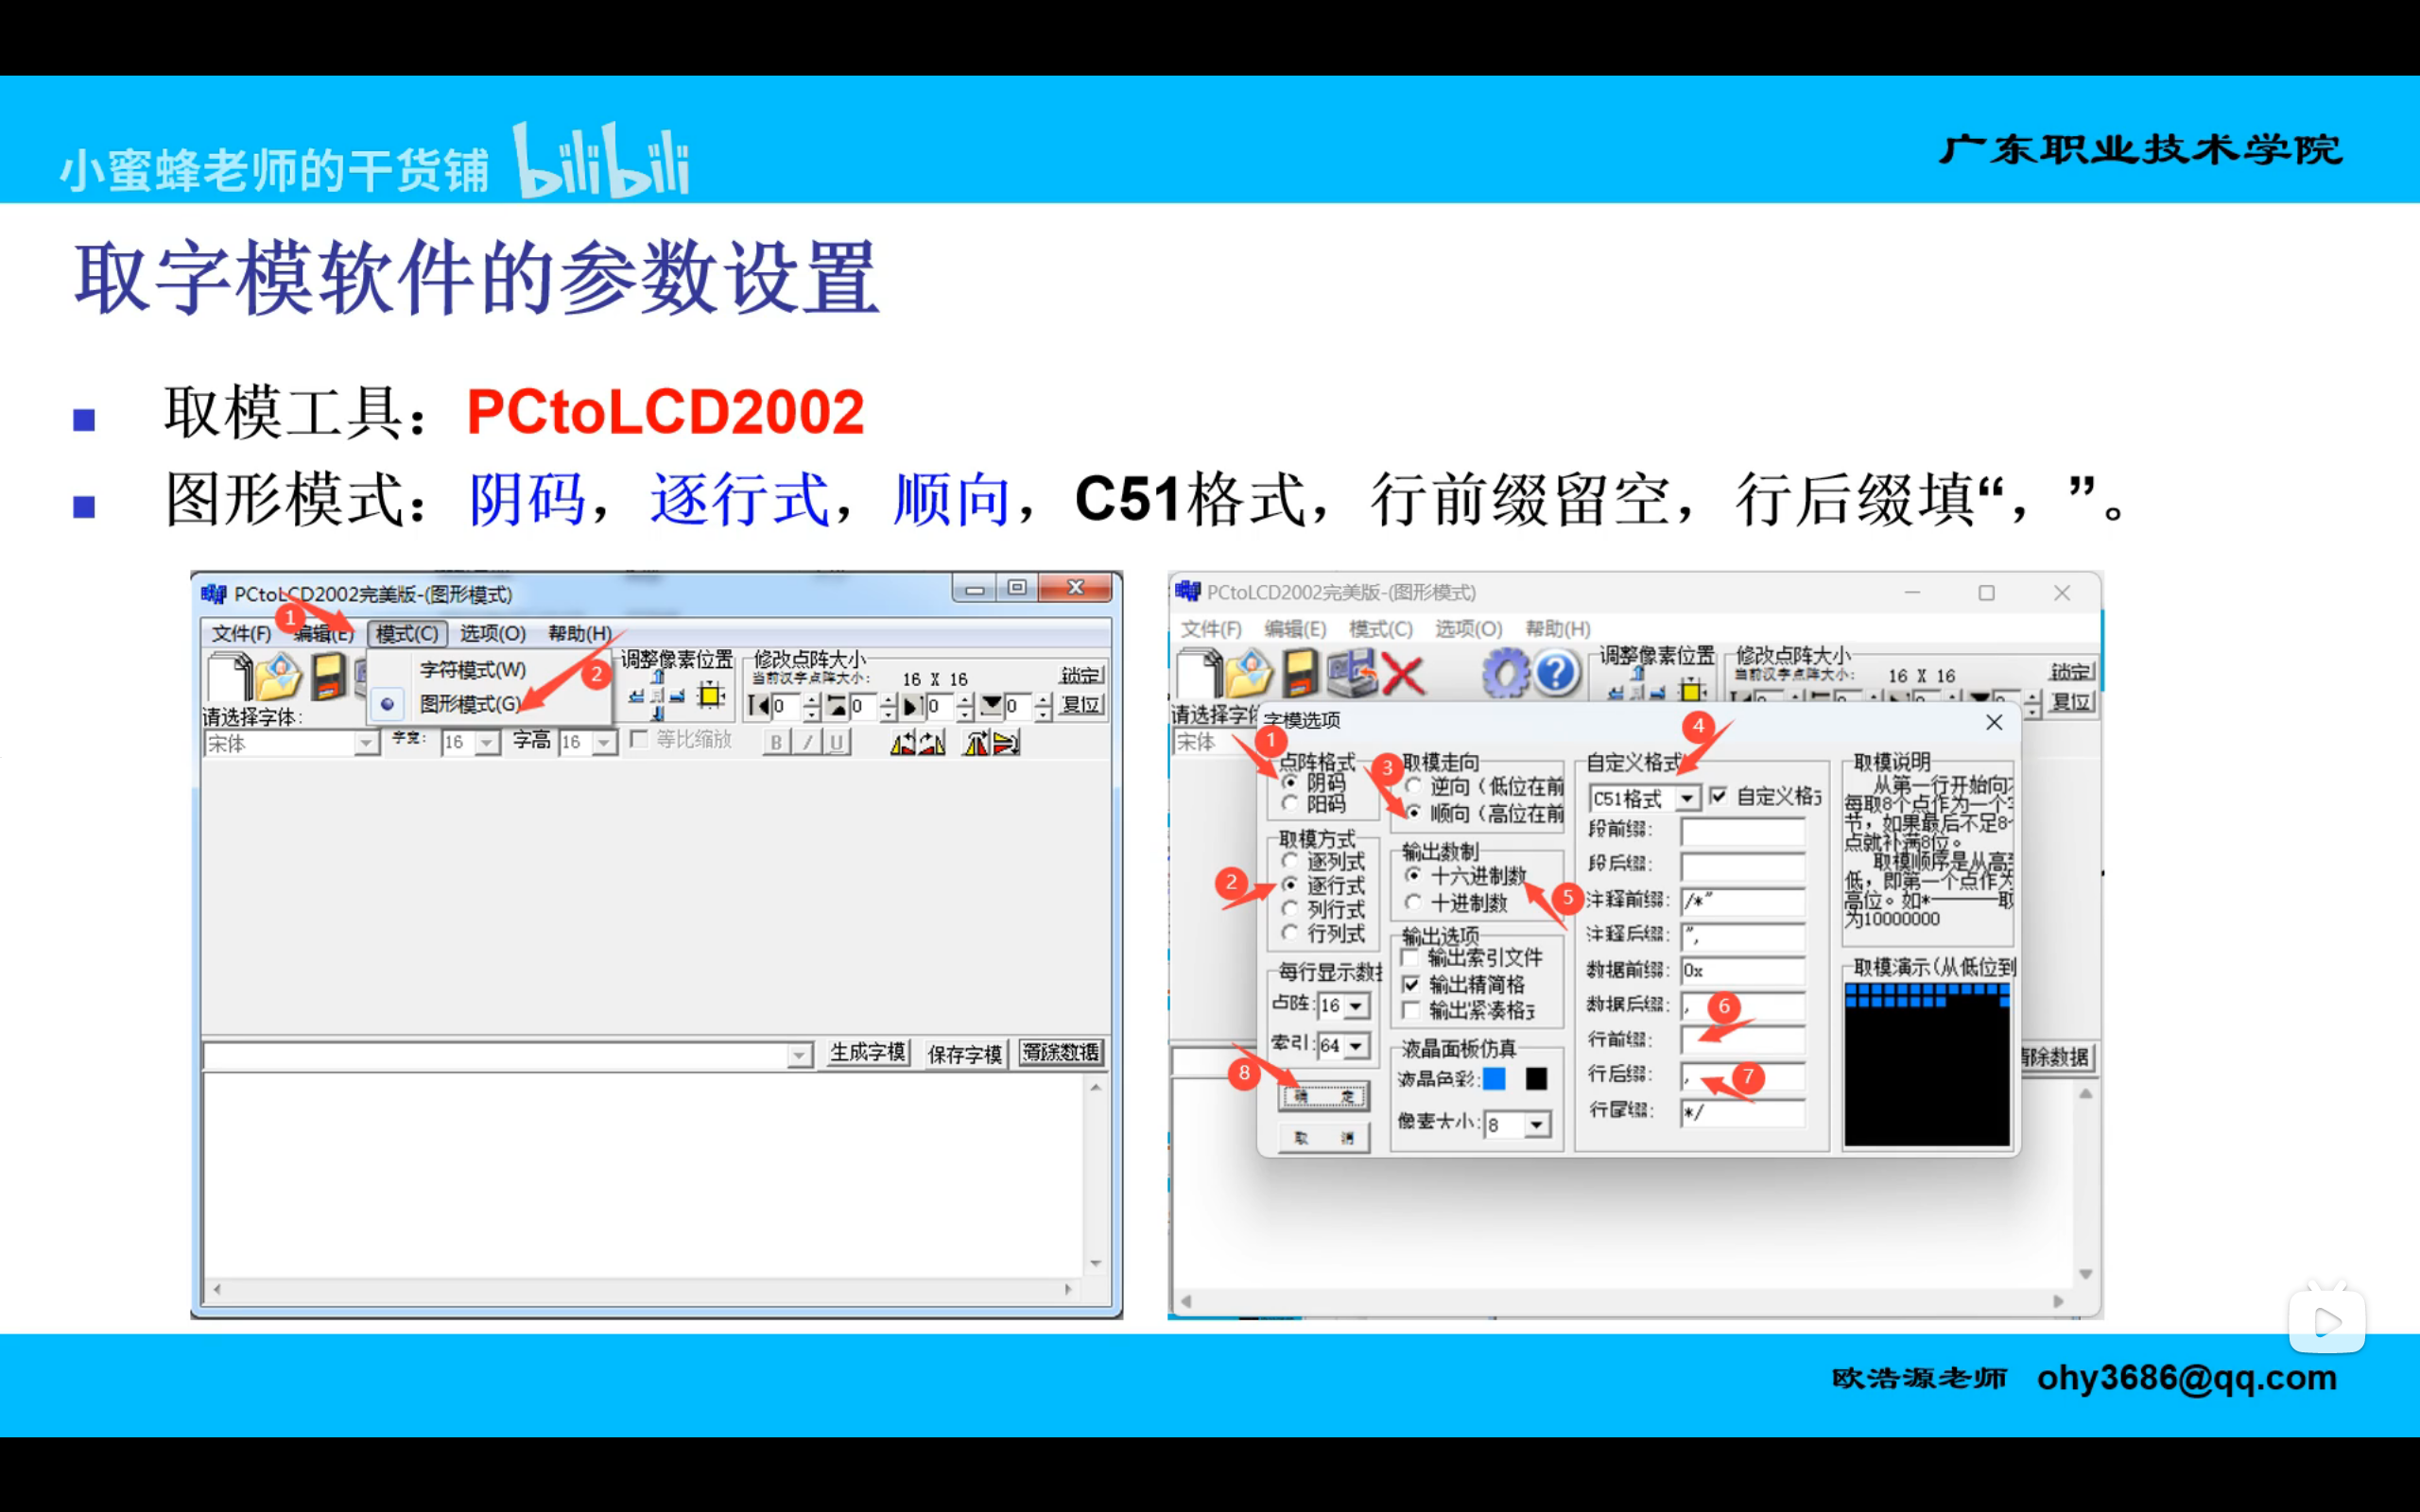
\includegraphics[width=\textwidth]{Figures/PCto.png}
    \caption{UP主的PCtoLCD2018 设置界面}
\end{figure}
需要注意的是，生成的字模数据格式必须与OLED驱动库要求的格式一致，否则可能无法正确显示图片。
对于不同的驱动库, 可能需要对生成的字模数据进行适当的调整或转换。此时可以参考该驱动库中类似drawBitmap的函数定义,
查看里面的函数实现, 以确定需要的数据格式和排列方式, 从而对生成的字模数据进行相应的修改。(如若看不懂,可以将该函数复制给AI,让它帮你分析一下需要什么样的数据格式)
\vspace{1em}

\textcolor{red}{\textbf{需要额外提醒的是}:读者对Adafruit SSD1306驱动库的drawBitmap函数进行
上述操作时会发现你最后会得出要使用阳码的结论,这是正确的。按照官方要求，本身就应该为阳码,但
不知为何UP主要使用阴码。对此作者也不是很明白，希望读者在使用过程中注意这一点。}
\newpage
\subsection{OLED显示中文汉字}
OLED显示中文汉字的步骤与显示图片类似，主要区别在于需要使用适合中文字符的字模数据。以下是具体步骤：
\begin{enumerate}
    \item 准备需要显示的中文汉字，可以是单个字符或字符串。
    \item 使用适合中文字符的字模工具（如PCtoLCD2018），设置正确的字模格式，将中文汉字转换为字模数据。UP主所设置的字模格式如下：
    \begin{figure}[h]
        \centering
        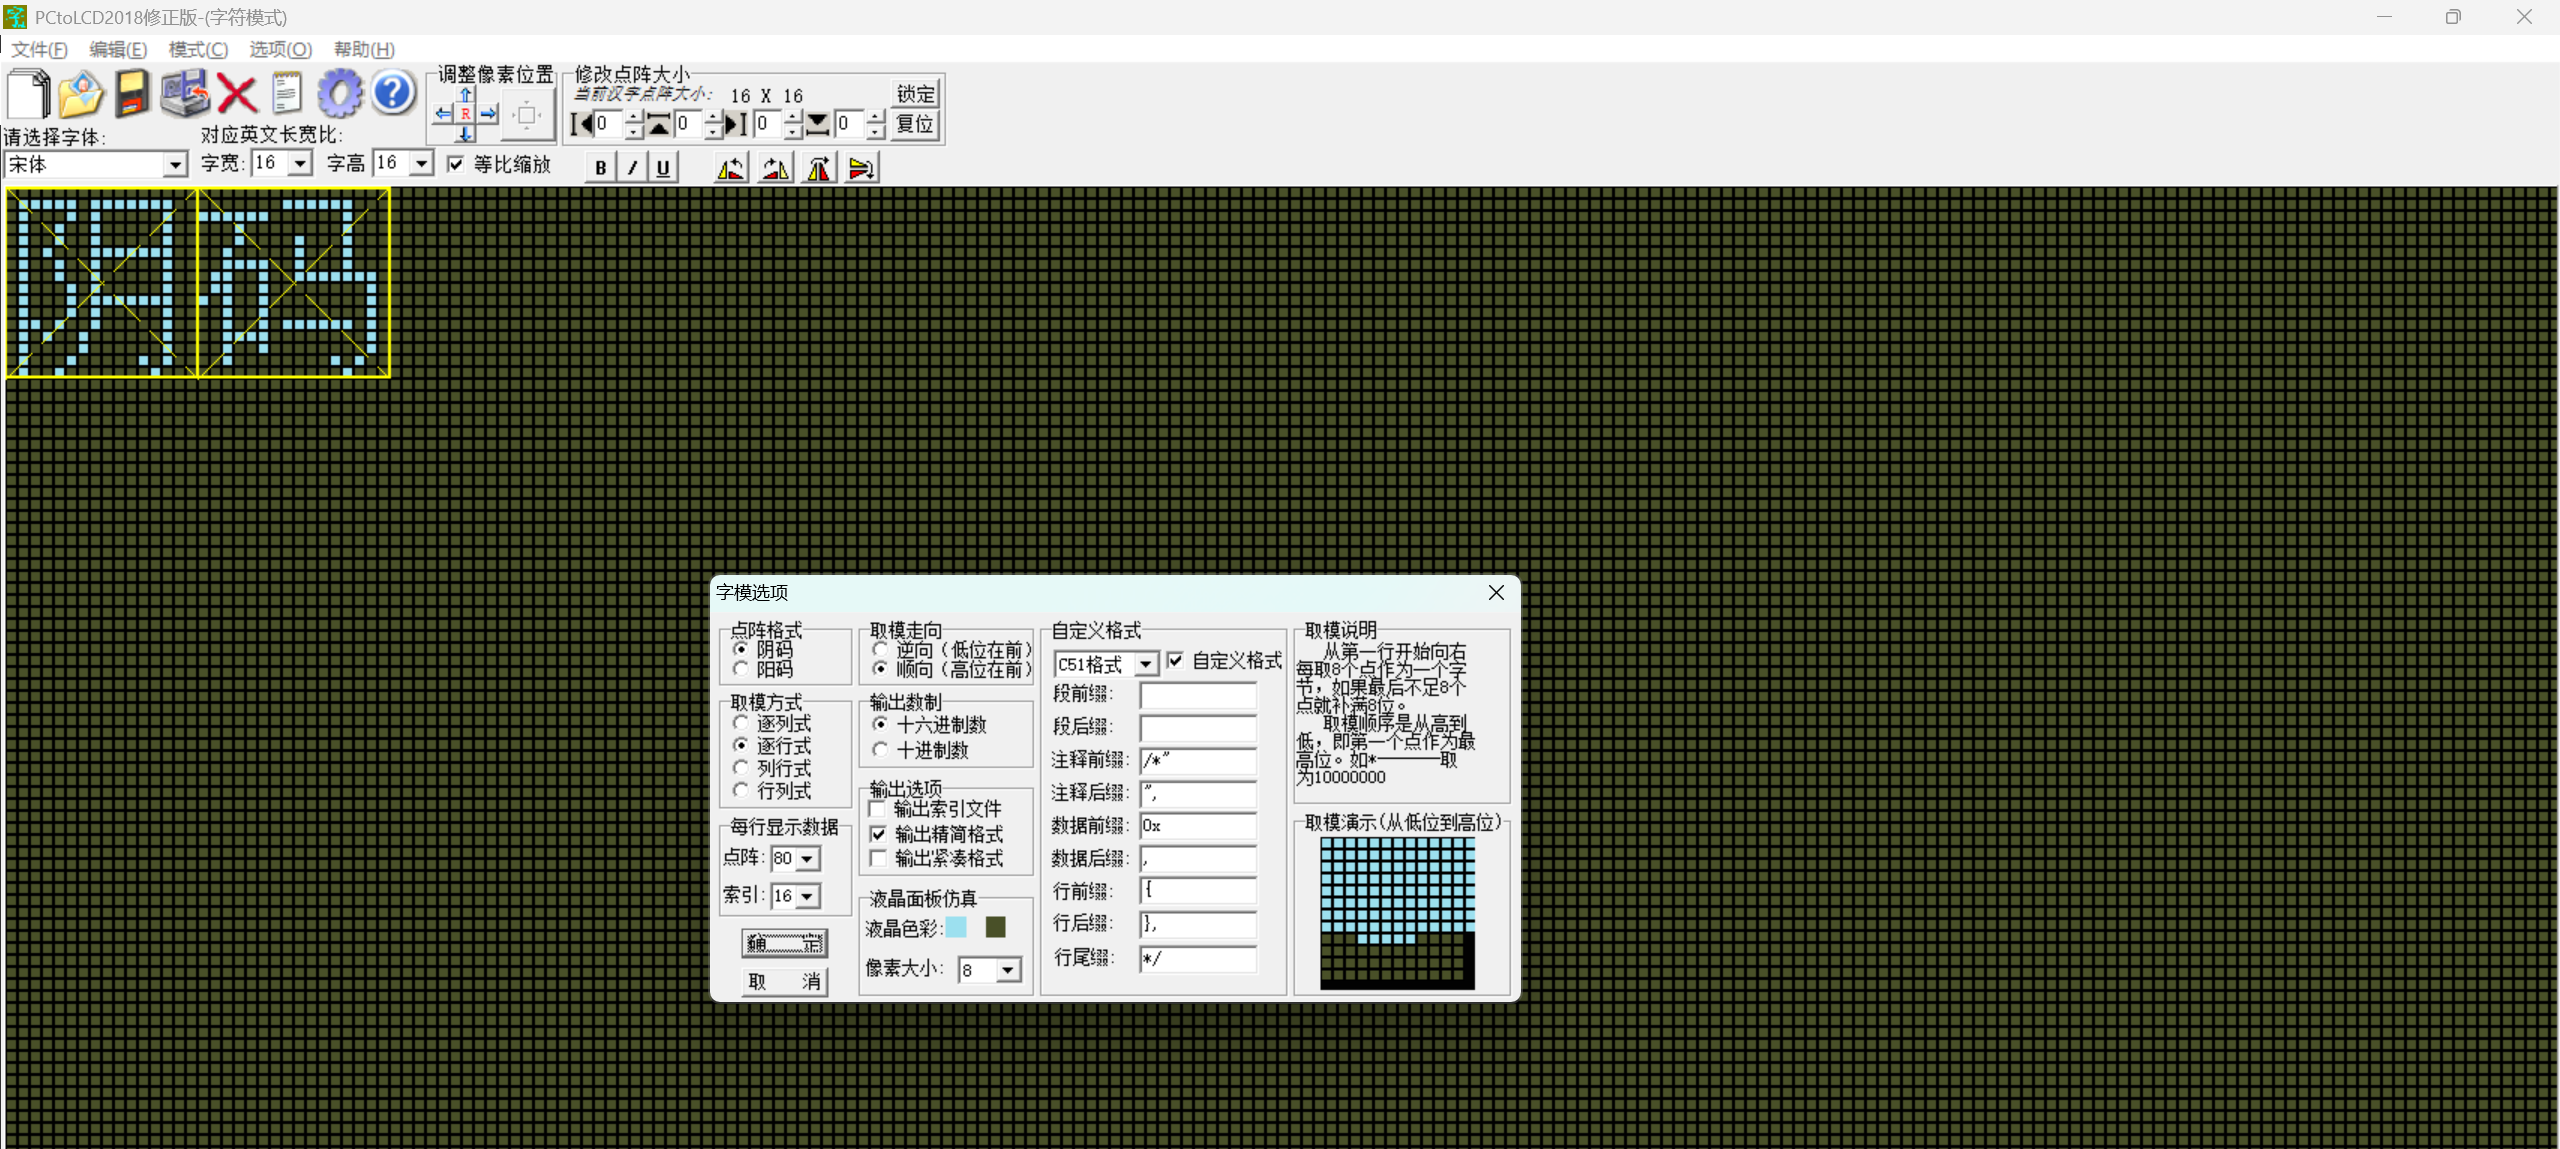
\includegraphics[width=\textwidth]{Figures/ChineseCharacters.png}
        \caption{UP主的PCtoLCD2018 设置界面-中文汉字}
    \end{figure}
    \item 将生成的字模数据复制到代码中，使用OLED驱动库提供的函数进行显示。通常，OLED驱动库会有专门的函数用于显示中文字符，确保使用正确的函数调用。
    \item 调整显示位置和字体大小，以确保中文汉字能够正确显示在OLED屏幕上。
\end{enumerate}
这是简单的汉字打印代码示例:
\begin{lstlisting}[language=C]
    void OLED_Show_Chinese(){
        oled.clearDisplay();
        /* Positive code*/
        oled.drawBitmap(0, 0, ziku[0], 16, 16, SSD1306_WHITE); 
        oled.drawBitmap(20, 0, ziku[1], 16, 16, SSD1306_WHITE);
        /* Negative code */
        oled.drawBitmap(0, 40, ziku[2], 16, 16, SSD1306_WHITE);
        oled.drawBitmap(20, 40, ziku[3], 16, 16, SSD1306_WHITE);
        oled.display();
    }
\end{lstlisting}
